\documentclass{article}
\usepackage{amsmath}
\usepackage{amsthm}
\usepackage{amssymb}
\usepackage{enumerate}
\usepackage{graphicx}
\usepackage{booktabs}

\begin{document}
    \title{MA4\_3 Exercise}
    \author{Wang Yue from CS Elite Class}
    \date{\today}

    \maketitle

    \section*{Exercise 4.3}

    \subsection*{50. $f(x) = x - \frac 1 6 x^2 - \frac 2 3 \ln x$}

    \begin{enumerate}[(a)]
        \item Find the vertical and horizontal asymptotes.

        % $f'(x) = 1 - \frac 1 3 x - \frac 2 {3x} = \frac{-x^2 + 3x - 2}{3x} = -\frac{(x - 1)(x - 2)}{3x}$

        $\because $$$\lim_{x \to \infty}(x - \frac 1 6 x^2 - \frac 2 3 \ln x) = -\infty$$

        $$\lim_{x \to 0^+}(x - \frac 1 6 x^2 - \frac 2 3 \ln x) = \infty$$

        $\therefore$ there is a vertical asymptote $x = 0$, but no horizontal asymptotes of $f$.

        \item Find the intervals of increase or decrease.

        $\because f'(x) = 1 - \frac 1 3 x - \frac 2 {3x} = \frac{-x^2 + 3x - 2}{3x} = -\frac{(x - 1)(x - 2)}{3x}$

        $\therefore$ we have the table below:

        \begin{table}[hbp]
            \begin{tabular}{@{}llllll@{}}
                \toprule
                intervals & $(0,1)$ & $1$ & $(1,2)$ & $2$ & $(2,\infty)$ \\ \midrule
                f' & - & 0 & + & 0 & - \\
                f & decreasing & local minimum & increasing & local maximum & decreasing \\ \bottomrule
            \end{tabular}
        \end{table}

        $\therefore $ increasing interval is $(1, 2)$ and decreasing intervals are $(0,1) , (2, \infty)$.

        \item Find the local maximum and minimum values.

        $\because $ by the conclusion of problem (b), $f$ attains its local minimum at $x = 1$ and local maximum at $x = 2$

        $\therefore $ the local minimum value is $f(1) = 1 - \frac 1 6 - 0 = \frac 5 6$, and the local maximum value is $f(2) = 2 - \frac 2 3 - \frac 2 3 \ln 2 = \frac 2 3 (2 - \ln 2)$

        \item Find the intervals of concavity and the inflection points.

        $\because f''(x) = \frac{\mathrm df'(x)}{\mathrm dx} = \frac{(-2x + 3)(3x) - 3(-x^2 + 3x - 2)}{9x^2} = \frac{2-x^2}{3x^2}$

        $\therefore$ we still have the table below:
    
    \begin{table}[hbp]
        \begin{tabular}{@{}llll@{}}
            \toprule
            intervals & $(0, \sqrt 2)$ & $\sqrt 2$ & $(\sqrt 2, \infty)$ \\ \midrule
            f'' & + & 0 & - \\
            concavity & \begin{tabular}[c]{@{}l@{}}concave\\ upward\end{tabular} & \begin{tabular}[c]{@{}l@{}}inflection\\ point\end{tabular} & \begin{tabular}[c]{@{}l@{}}concave\\ downward\end{tabular} \\ \bottomrule
        \end{tabular}
    \end{table}
        \item Use the information from parts (a)-(d) to sketch the graph of $f$.

        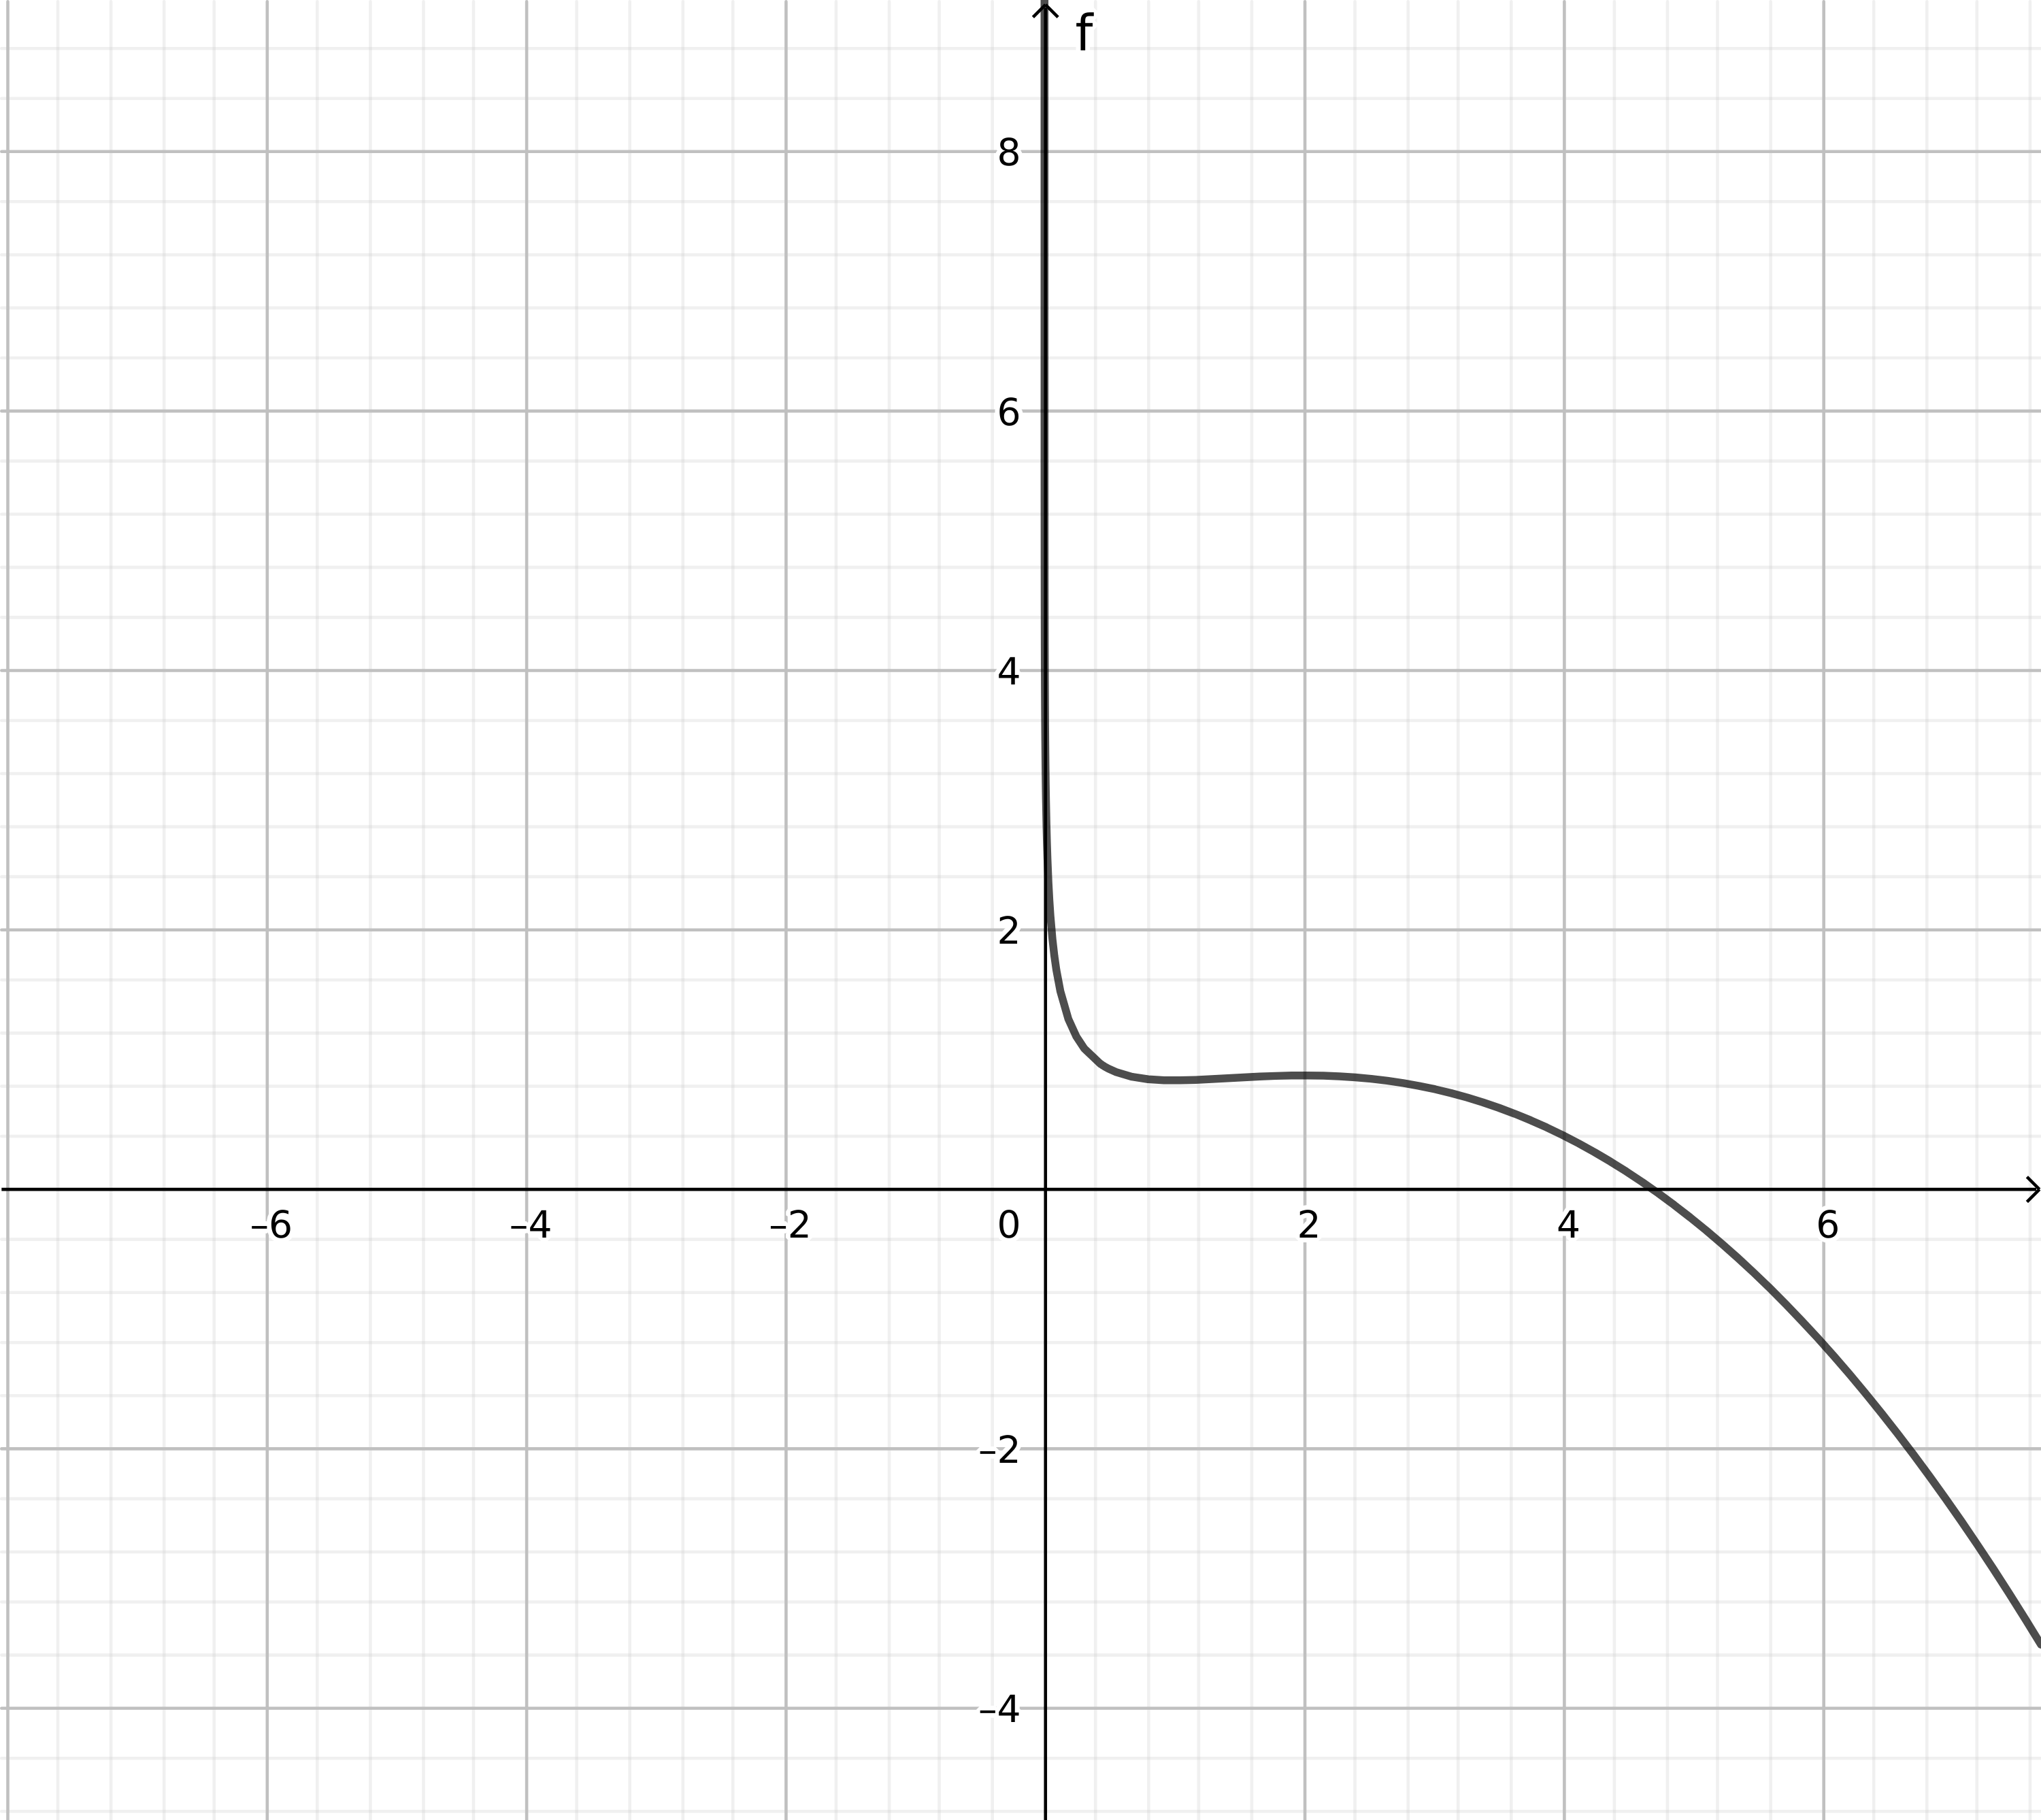
\includegraphics[scale = 0.6]{50.png}

    \end{enumerate}

    \subsection*{81. Prove that if $(c, f(c))$ is a point of inflection of the graph of $f$ and $f''$ exists in an open interval that contains $c$, then $f''(c) = 0$.}

    \begin{proof}
        Without loss of generality, let the open interval be $(a, b)$ with c inside.

        Introduce a new function $$F(x) = \left\{ \begin{array}{ll}
            \lim_{x \to a^+} f(x) & \textrm{if $x = a$} \\
            f(x) & \textrm{if $a < x < b$} \\
            \lim_{x \to b^-} f(x) & \textrm{if $x = b$}
        \end{array} \right.$$

        $\because f''$ exists in $(a,b)$

        $\therefore f'$ is differentiable in $(a,b)$ 

        $\therefore F'$ is differentiable in $(a,b)$ and continuous on $[a,b]$ 

        $\because (c, f(c))$ is an inflection point in $(a,b)$

        $\therefore f'(x)$ attains local maximum or minimum at $x = c$ in $(a,b)$

        $\therefore $ by the Rolle Theorem, $f''(c) = 0$
    \end{proof}

    \subsection*{82. Show that if $f(x) = x^4$, then $f''(0) = 0$, but $(0, 0)$ is not an inflection point of the graph of $f$.}

    \begin{proof}
        $\because f(0) = 0, f'(x) = 4x^3, f''(x) = 12x^2$

        $\therefore f''(0) = 12 \times 0 = 0$

        $\because$ when $x < 0$, $f''(x) = 12x^2 > 0$; when $x > 0$, $f''(x) = 12x^2 > 0$

        $\therefore f(x)$ is both concave upward on $(-\infty, 0)$ and $(0, \infty)$ 

        $\therefore$ $(0,0)$ is not an inflection point though $f''(0) = 0$
    \end{proof}

    \subsection*{83. Show that the function $g(x) = x |x|$ has an inflection point at $(0,0)$ but $g''(0)$ does not exist.}
    
    \begin{proof}
        $\because g(x) = \left\{ \begin{array}{ll}
            x^2 & \textrm{if $x > 0$} \\
            0 & \textrm{if $x = 0$} \\
            -x^2 & \textrm{if $x < 0$}
        \end{array} \right.$

        $\therefore g'(x) = \left\{ \begin{array}{ll}
            2x & \textrm{if $x > 0$} \\
            0 & \textrm{if $x = 0$} \\
            -2x & \textrm{if $x < 0$}
        \end{array} \right.$

        $\therefore g''(x) = \left\{ \begin{array}{ll}
            2 & \textrm{if $x > 0$} \\
            -2 &\textrm{if $x < 0$}
        \end{array} \right.$

        $\because$ when $x \in (-\infty, 0), g''(x) < 0; x \in (0, \infty), f''(x) > 0$

        $\therefore g(x)$ is concave downward in $(-\infty, 0)$ and concave upward $(0, \infty)$

        $\therefore (0, 0)$ is an inflection point.

        However, $\because \lim_{x \to 0^-}\frac{g'(x) - g'(0)}{x - 0} = -2 \not = \lim_{x \to 0^+}\frac{g'(x) - g'(0)}{x - 0} = 2$

        $\therefore g''(0)$ does not exist.

    \end{proof}
\end{document}